\chapter{Results}
Evaluating the performance of machine learning models is crucial for understanding their effectiveness and limitations in practical applications. In this study, the developed models were tested on user data to assess their accuracy and generalization capabilities. Various factors, such as feature representation, input sequence length, and class balance, can significantly influence model performance.

\section{Model performance on user data}
This section focuses on the results of testing the collection of models that achieved the best performance during validation. It aims to show how this solution performs on the unseen test dataset and highlights the large differences between individual models within the collection of models.

\subsection{Methodology}
The results below were calculated as an average of each model's performance on sequences of characters of the same length as those on which the model was trained.
The results presented below were obtained using the combination of input features listed in table \ref{table:hyperparams}, which yielded the best performance during model validation. The impact of each hyperparameter choice is discussed separately in dedicated subsections and compared using the testing provided by users. It is important to note that due to the large number of possible configurations, as well as the limited computing power that was available, not all combinations were tested.

\begin{center}
	\begin{table}[H]
		
\begin{center}
	\begin{tabular}{ |c|c|} 
		\hline
		Hyperparameter & Value \\
		\hline
		Input length & \textit{40} \\ 
		\hline
		Edge encoding method & \textit{Two values per node} \\		
		\hline 
		Character encoding method & \textit{Normalized Base Letter Encoding} \\		 
		\hline
		Decision threshold & \textit{0.8} \\
		\hline
	\end{tabular}
\end{center}
	\caption{Input feature choices.}
	\label{table:hyperparams}
	\end{table}
\end{center}


\subsection{FAR and FRR scores}
The table below presents the false authentication rate and false acceptance rate for all models. The motivation for using these metrics was discussed in subsection \ref{FAR_FRR_theory}.

\begin{center}
\begin{table}[H]
\begin{center}
	\begin{tabular}{ |c|c|c| } 
		\hline
		User ID & False Acceptance Rate & False Rejection Rate \\
		\hline
		21 & 0.242 & 0.119 \\
		\hline
		22 & 0.063 & 0.000 \\
		\hline
		23 & 0.200 & 0.479 \\
		\hline
		24 & 0.042 & 0.658 \\
		\hline
		25 & 0.050 & 0.015 \\
		\hline
		26 & 0.086 & 0.032 \\
		\hline
		40 & 0.080 & 0.459 \\
		\hline
		41 & 0.057 & 0.355 \\
		\hline
		42 & 0.135 & 0.379 \\
		\hline
		60 & 0.083 & 0.608 \\
		\hline
		61 & 0.066 & 0.065 \\
		\hline
		62 & 0.044 & 0.032 \\
		\hline
		81 & 0.086 & 0.802 \\
		\hline
		82 & 0.045 & 0.024 \\
		\hline
		83 & 0.116 & 0.322 \\
		\hline
		85 & 0.128 & 0.144 \\
		\hline
		86 & 0.037 & 0.000 \\
		\hline
		\hline
		Average & 0.092 & 0.264 \\
		\hline
	\end{tabular}
\end{center}
\caption{FAR and FRR scores for all models.}
\label{table:FAR_FRR_base}
\end{table}
\end{center}

The same data can be visualized as a plot of the false acceptance rate versus the false rejection rate, as shown in figure \ref{fig:frr_vs_far_all_models_base}. 

\begin{figure}[H]
	\centering
	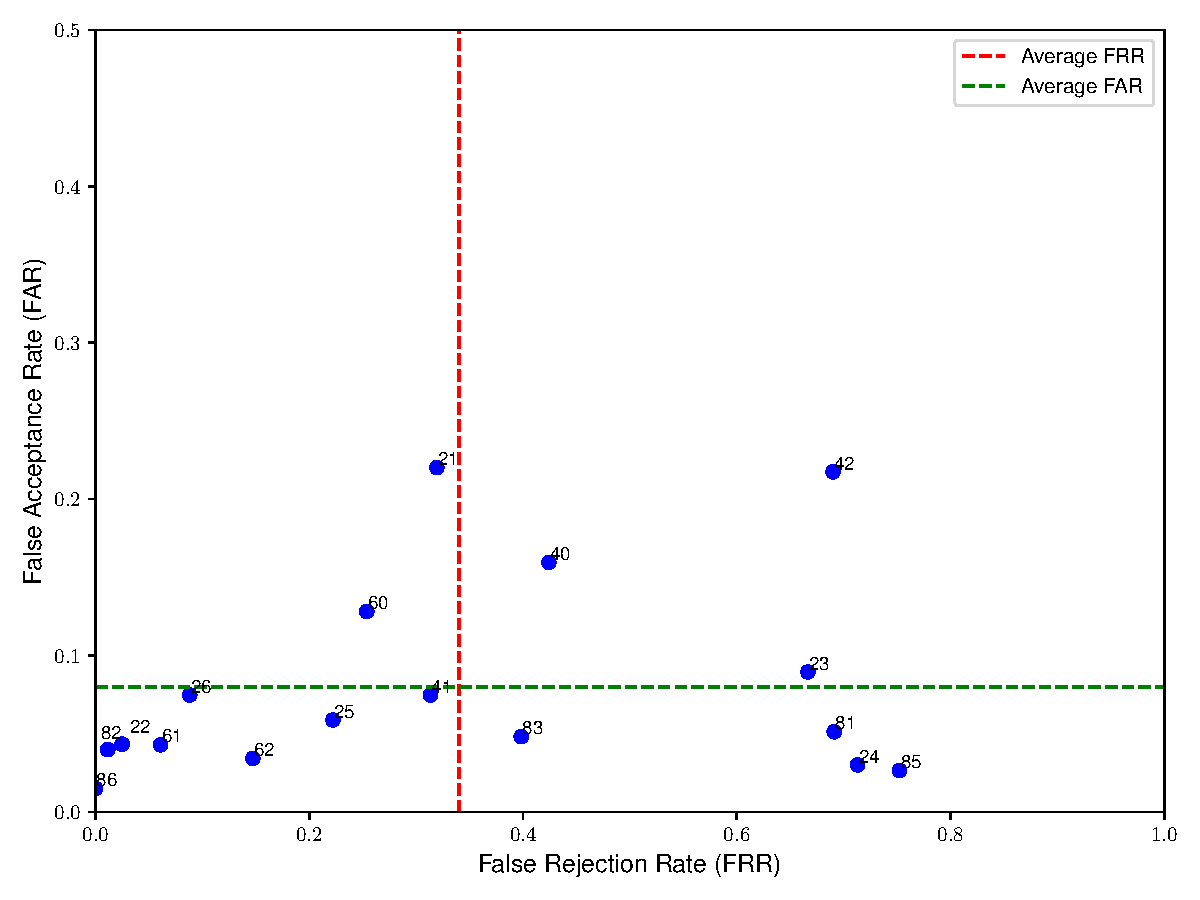
\includegraphics[width=\textwidth]{images/far_vs_frr.pdf} 	
	\caption{False acceptance rate versus False rejection rate.}
	\label{fig:frr_vs_far_all_models_base}
\end{figure}

Figure \ref{fig:frr_vs_far_all_models_base} demonstrates a large discrepancy between the models. At the same threshold level, some models were able to achieve a FAR and FRR score below 10\%, while others failed to recognize more than half of the examples in the positive class. \\
This first group consists of models for users 86, 62, 82, 25, 26, and 61. These models were able to effectively learn and generalize the test dataset well.
The other major group of models was those with an unacceptably high FAR exceeding 45\% and a below-average FAR score. These group includes models for users 81, 24, 60, 40 and 23. The reason for such high FAR could be twofold, either the models simply failed to generalize to unseen positive examples, or they did but with a lower confidence level than the established threshold. Other models have varying performance and are difficult to categorize into coherent groups.

\subsection{Equal Error Rate} \label{subsec_eer}
To calculate the equal error rate, the decision threshold needs to be adjusted, which can be performed globally, for all models or individually at a per--model level. Both methods of calculating this metric were analyzed.

The global EER was calculated to illustrate the performance of the entire collection with a single value.
\begin{itemize}
	\item[] Equal Error Rate: 0.157
	\item[] Threshold: 0.20
\end{itemize}
A low decision threshold was necessary to achieve an equal error rate. This suggests that most models are unable to recognize positive examples with a high level of confidence. Such a low value would not be practical in an applied setting and within the context of the system developed in this project. 

The per-model EER can be used to examine the differences among the models.
It is calculated by finding the equal error rate decision threshold for each model separately.
The results are shown in table \ref{table:EER_separate}.
\begin{center}
	\begin{table}[H]
		\begin{center}
			\begin{tabular}{ |c|c|c| } 
				\hline
				User ID & Equal Error Rate & Decision threshold \\
				\hline
				\hline
				21 & 0.124 & 0.95 \\
				\hline
				22 & 0.026 & 0.95 \\
				\hline
				23 & 0.245 & 0.40 \\
				\hline
				24 & 0.270 & 0.05 \\
				\hline
				25 & 0.037 & 0.85 \\
				\hline
				26 & 0.059 & 0.80 \\
				\hline
				40 & 0.200 & 0.05 \\
				\hline
				41 & 0.081 & 0.35 \\
				\hline
				42 & 0.163 & 0.45 \\
				\hline
				60 & 0.176 & 0.05 \\
				\hline
				61 & 0.066 & 0.80 \\
				\hline
				62 & 0.038 & 0.85 \\
				\hline
				81 & 0.392 & 0.05 \\
				\hline
				82 & 0.026 & 0.95 \\
				\hline
				83 & 0.220 & 0.05 \\
				\hline
				85 & 0.131 & 0.75 \\
				\hline
				86 & 0.028 & 0.90 \\
				\hline
				\hline
				Average & 0.133 & -- \\
				\hline
			\end{tabular}
		\end{center}
		\caption{Per model equal error rate.}
		\label{table:EER_separate}
	\end{table}
\end{center}

Table \ref{table:EER_separate} illustrates the differences in the models' ability to generalize unseen positive examples. This is further demonstrated by examining the changes in FAR and FRR scores with respect to the decision threshold, which is show in figure \ref{fig:far_ffr_all_thresholds}. 

\begin{figure}[H]
	\centering
	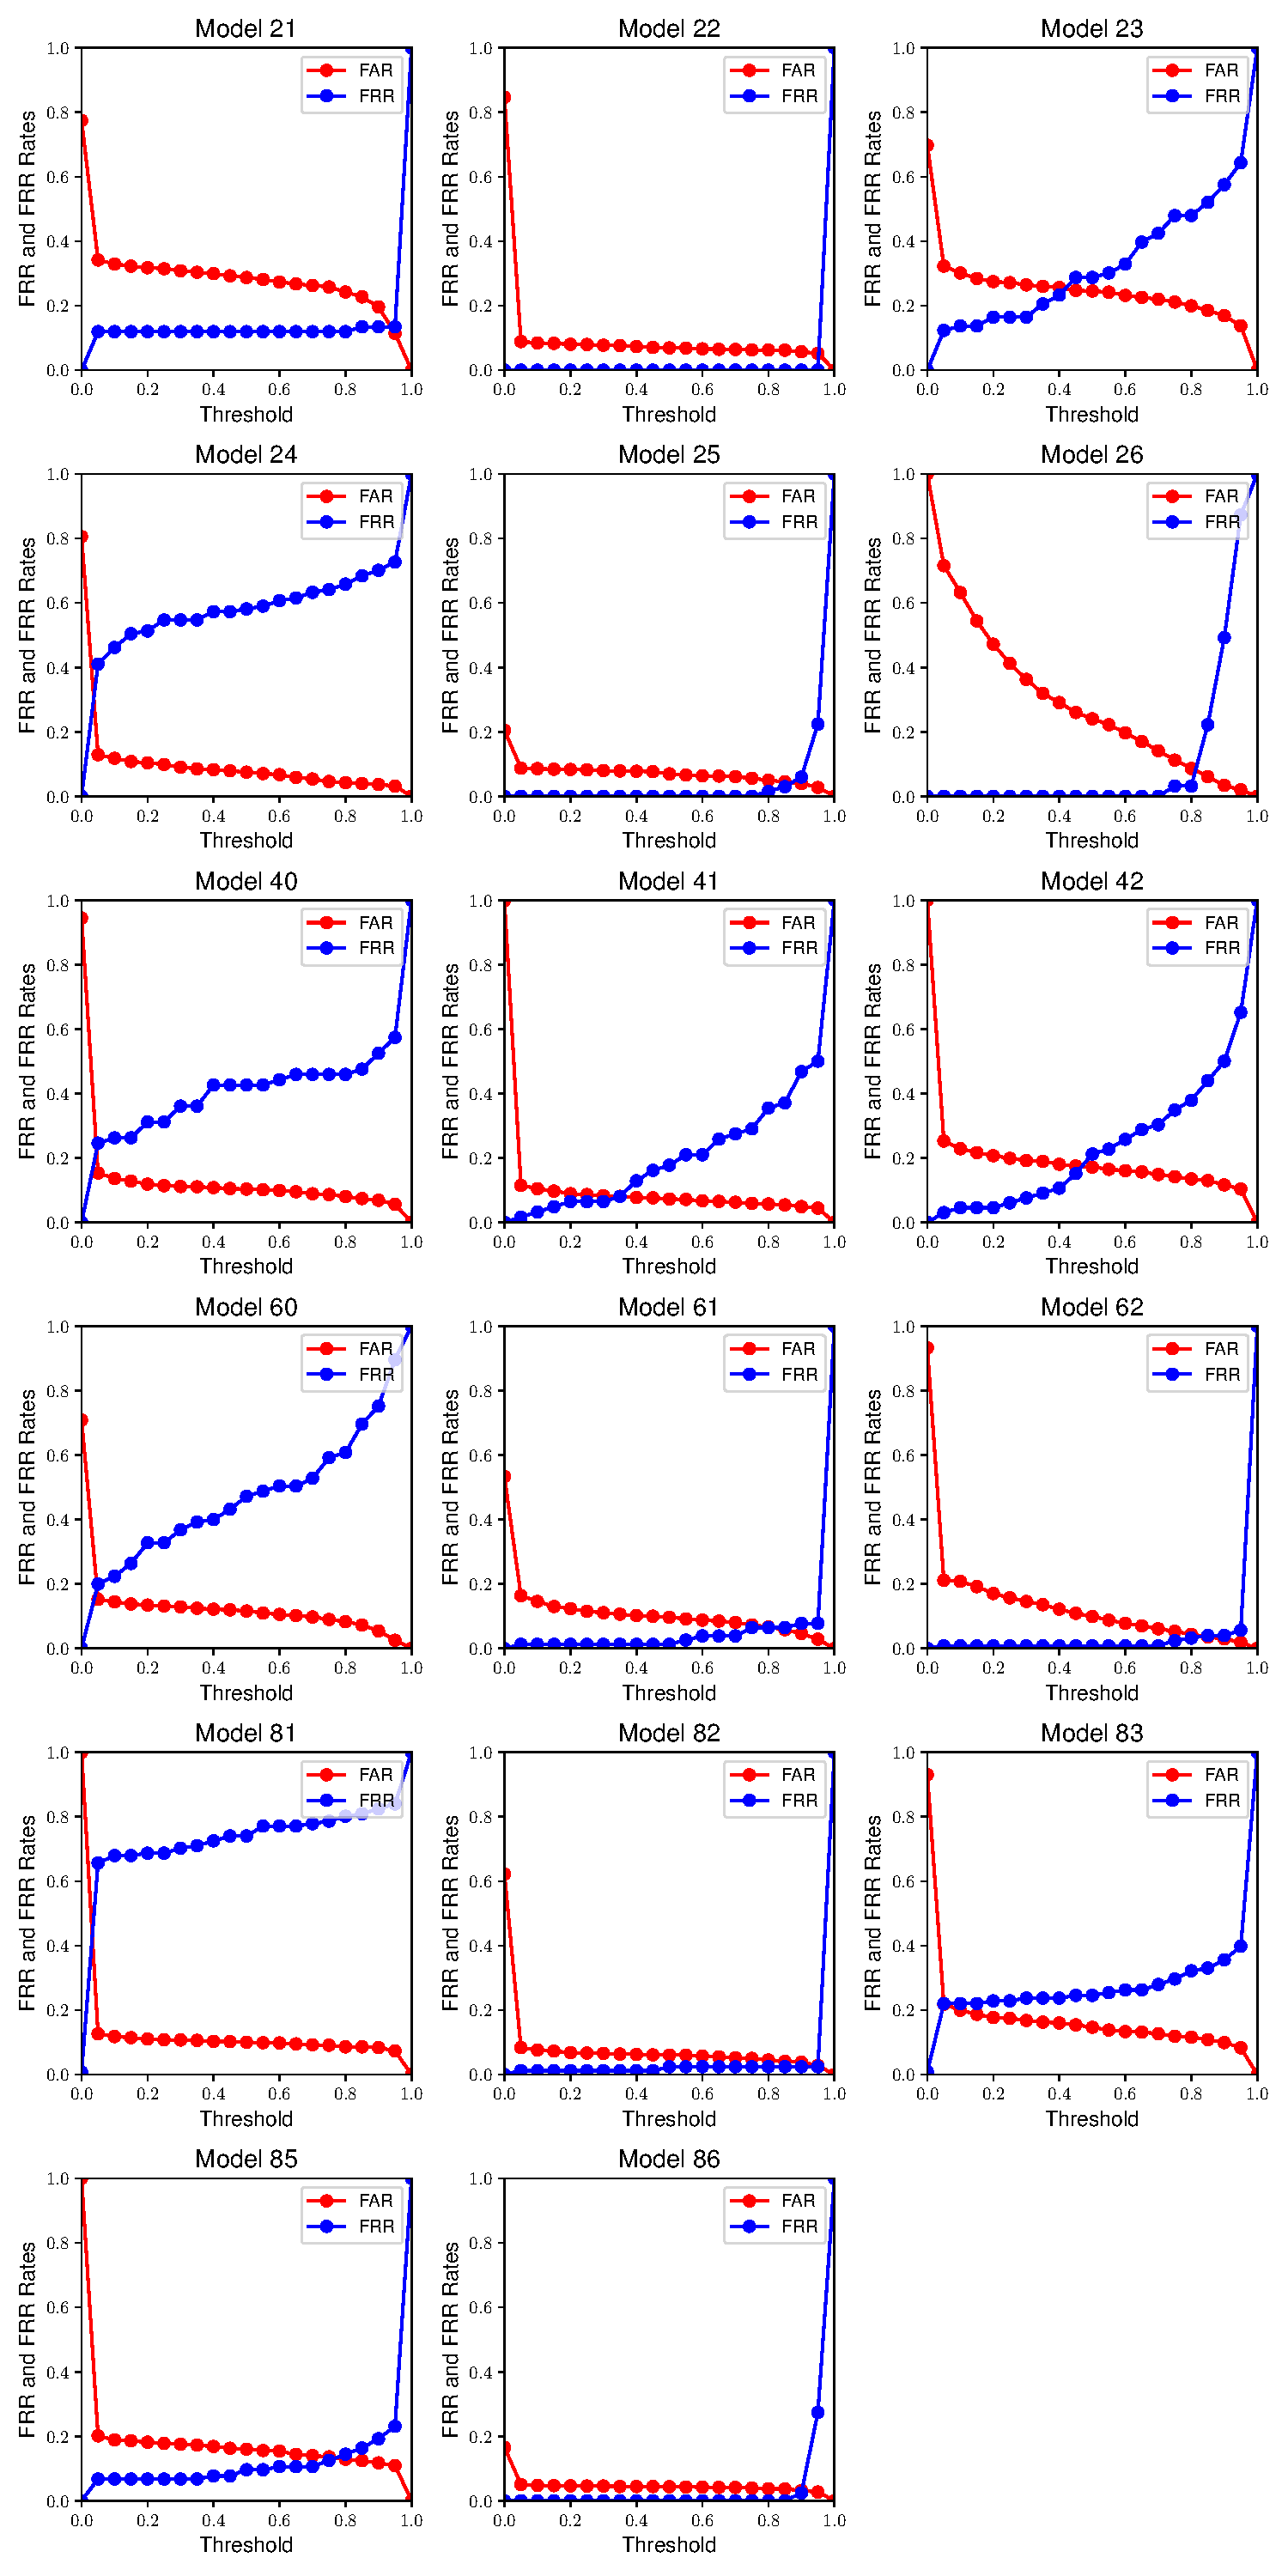
\includegraphics[width=.8\textwidth]{images/far_frr_curves_all_models_subplots.pdf} % Replace 'example.pdf' with your PDF file name
	\caption{Change of FAR and FRR score with respect to decision threshold.}
	\label{fig:far_ffr_all_thresholds}
\end{figure}

These plots show the relationship between FAR, FRR, and the decision threshold in more detail. The point at which the two lines cross is the EER. It is worth noting the large variation in the threshold at which the EER is achieved. Models for users 21, 22, 25, 26, 61, 62, 82, 85, and 86 reach an equal error rate at or above a threshold of 0.8, which indicates a high degree of confidence in the prediction of positive class. These models have a lower EER than models with lower threshold values. To illustrate this, table \ref{table:EER_separate}, sorted by EER, is given below.

\begin{center}
	\begin{table}[H]
		\begin{center}
			\begin{tabular}{ |c|c|c| } 
				\hline
				User ID & Equal Error Rate & Decision threshold \\
				\hline
				\hline
				22 & 0.026 & 0.95 \\
				\hline
				82 & 0.026 & 0.95 \\
				\hline
				86 & 0.028 & 0.9 \\
				\hline
				25 & 0.037 & 0.85 \\
				\hline
				62 & 0.038 & 0.85 \\
				\hline
				26 & 0.059 & 0.8 \\
				\hline
				61 & 0.066 & 0.8 \\
				\hline
				41 & 0.081 & 0.35 \\
				\hline
				21 & 0.124 & 0.95 \\
				\hline
				85 & 0.131 & 0.75 \\
				\hline
				42 & 0.163 & 0.45 \\
				\hline
				60 & 0.176 & 0.05 \\
				\hline
				40 & 0.2 & 0.05 \\
				\hline
				83 & 0.22 & 0.05 \\
				\hline
				23 & 0.245 & 0.4 \\
				\hline
				24 & 0.27 & 0.05 \\
				\hline
				81 & 0.392 & 0.05 \\
				\hline
			\end{tabular}
		\end{center}
		\caption{Sorted per model equal error rate.}
		\label{table:EER_separate_sorted}
	\end{table}
\end{center}

An outlier in this trend is model 41, which achieves an equal error rate of 8.1\% at a 0.35 decision threshold, outperforming models with much higher decision thresholds. Outliers like this suggest that a better approach than choosing one decision threshold could be to determine them on a per-model basis. Such a threshold could be chosen once, on some portion of the user training data through cross-validation, although such an approach would lengthen the training process. Alternatively, such a value could be adjusted dynamically, based on how often a user fails to be authenticated using the model. Such considerations could be an area of further research as they fall outside the scope of this project.
Additionally, because a global decision results in poor performance for otherwise well-performing models, it can be concluded that the average per-model EER is a better metric to use than the global EER and, as such, it will be used in the rest of this chapter.
Another interesting example is model 21, for which the FRR is almost constant, at a value of around 12\%. This indicates that all examples are recognized with a high degree of confidence, except for those 12\%, which may indicate that the user changes writing styles for part of the final input or that the training data failed to capture some characteristic of the writing style.

\subsection{Confusion matrix for all users}
To evaluate each model's performance, each model was tested using the input of every user. The results of this test are shown in figure \ref{fig:all_models_5_len40}. The values in this matrix represent the percentage of examples classified as positive. It is important to note that the values in this matrix have a different interpretation depending on their position. The values on the diagonal represent the percentage of correctly classified positive examples (True Positives) -- the recall of the model. In an ideal classifier, these values would equal 100. The values outside the diagonal represent the percentage of incorrectly classified negative examples (False Positives). In an ideal classifier, these values would equal 0.

\begin{figure}[H]
	\centering
	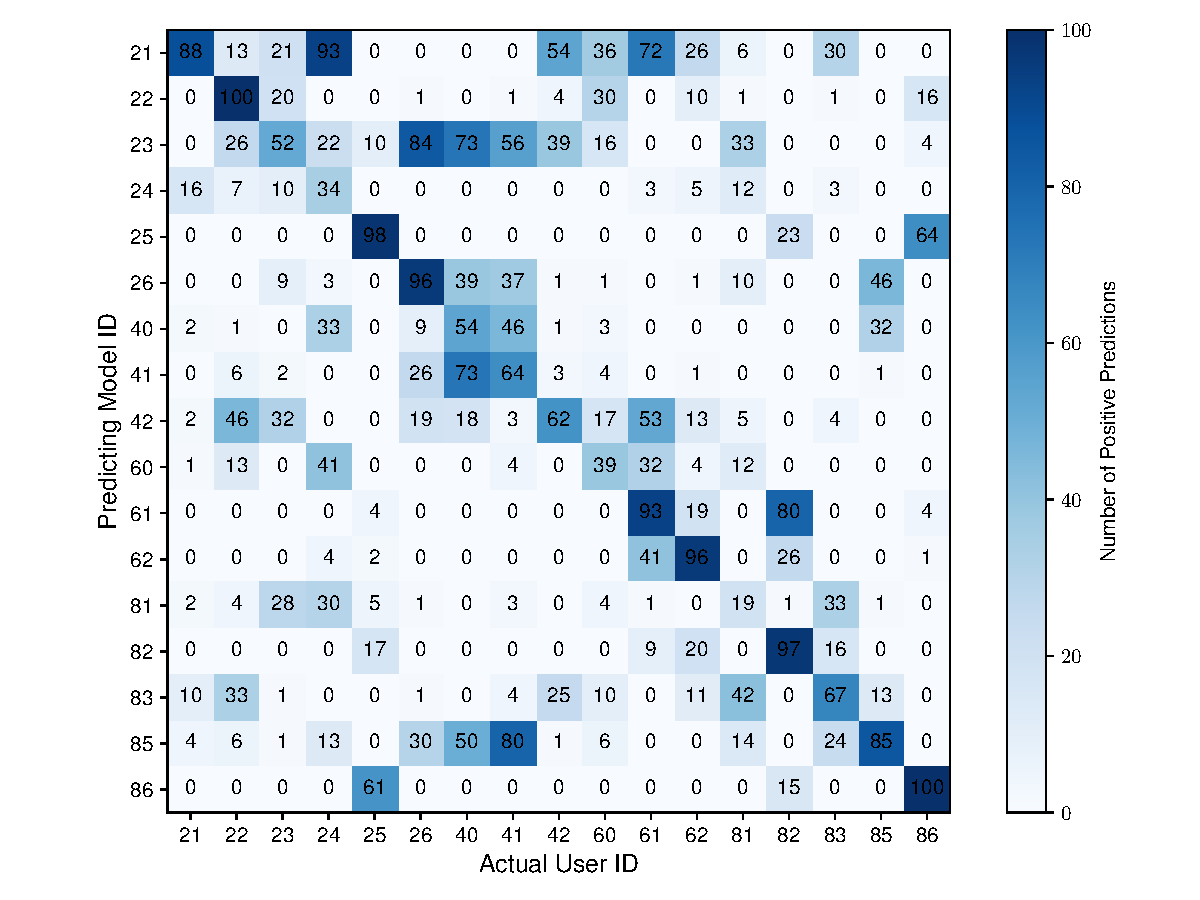
\includegraphics[width=\textwidth]{images/all_models_5_len40.pdf}
	\caption{Matrix showing the percentage of examples classified as positive for all model--user pairs.}
	\label{fig:all_models_5_len40}
\end{figure}

Figure \ref{fig:all_models_5_len40} illustrates the different types of errors made by individual models. Specifically, it highlights which users share similarities, leading to confusion in model predictions. For example, models for users 25 and 86 perform very well for all inputs except for each other. However, this is not true for all models, as the model for user 61 makes mistakes when classifying the input for user 82. The inverse is not observed, as the model for user 82 does not misclassify user 61's data at a higher rate than others.

\section{Input features}
This section compares the impact of input encodings on the final model performance, as measured by the average FAR and FRR, as well as the average per-model EER value. The impact of these changes was measured by changing only a single hyperparameter, while all others remained the same, as shown in table \ref{table:hyperparams}. The results shown below compare performance on the testing dataset, allowing these values can be contrasted with what was discussed in the previous section. As mentioned previously, this is not how these features were selected.

\subsection{Input sequence length}
The theoretical impact of input length, as discussed in the section on graph creation, suggests that an optimal sequence length exists. Making the sequence shorter would result in graphs that do not have enough structure, for example, a chain of nodes or not enough edge data to make the correct prediction possible. Making the sequence longer would result in a graph that is too dense, or it would cause the averages calculated per node to become too aggregated.


\begin{center}
	\begin{table}[H]
		\begin{center}
			\begin{tabular}{ |c|c|c|c| } 
				\hline
				Input sequence length & FAR & FRR & EER \\
				\hline
				30 & 0.101 & 0.332 & 0.180 \\
				\hline
				40 & 0.092 & 0.264 & 0.133 \\
				\hline
				50 & 0.098 & 0.232 & 0.135 \\
				\hline
				60 & 0.079 & 0.307 & 0.158 \\
				\hline
				70 & 0.083 & 0.391 & 0.176 \\
				\hline
			\end{tabular}
		\end{center}
		\caption{Comparison of performance with different lengths of input sequence.}
		\label{table:len_vs_perf}
	\end{table}
\end{center}


Table \ref{table:len_vs_perf} partially supports the theoretical expectation, as models trained on input sequences of length 30, 60 and 70 achieve much higher EER scores than those trained with lengths of 40 and 50. There is a very small difference in the performance of these model collections on the aggregated metrics. 
With the difference in the EER scores being this low, it is unclear which collection of models performed better on the testing dataset.
However, interesting differences appear when compared on a per-model basis, as the changes in models were not uniform. The impact of three selected models is shown in figure \ref{fig:selected_frr_vs_far}. 

\begin{figure}[H]
	\centering
	\subfloat[Plots for input of length 40]{
		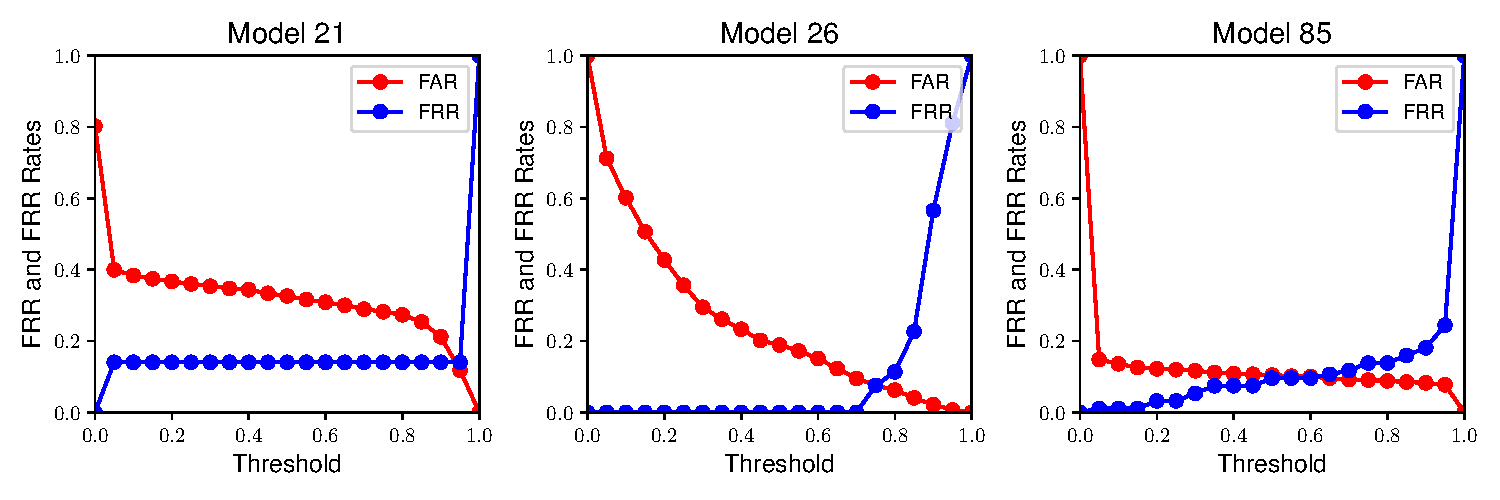
\includegraphics[width=\textwidth]{images/selected_far_vs_frr_len40.pdf}
	}

	\subfloat[Plots for input of length 50]{
		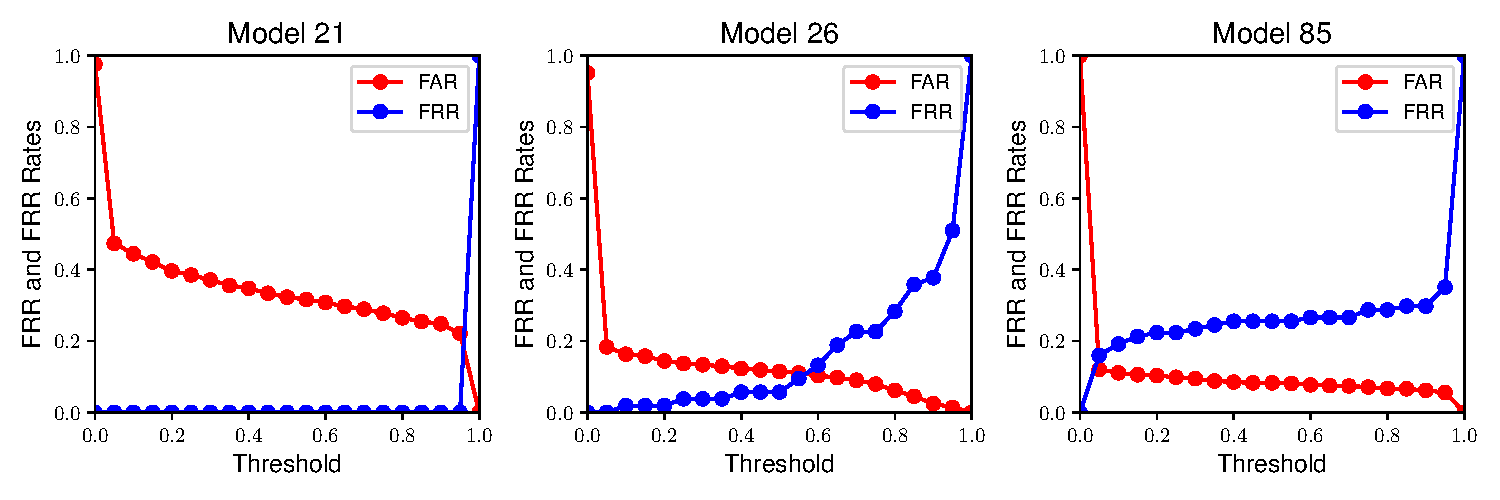
\includegraphics[width=\textwidth]{images/selected_far_vs_frr_len50.pdf}
	}
	\caption{Comparison of selected FAR and FRR plots for different input lengths}%
	\label{fig:selected_frr_vs_far}%
\end{figure}

The model for user 21 shows a clear improvement as the unrecognized examples discussed in subsection \ref{subsec_eer} are now correctly classified. Conversely, the model for user 26 now classifies its positive examples with less confidence and showed an increase in EER from 5.9\% to 10.2\%. For model 85 the change in length did not impact the EER. However, it moved the decision threshold significantly.
What these comparisons demonstrate is that it is hard to reason about model performance across different input sequence lengths and a small change has a large impact even on a per-model basis.

\subsection{Character encoding}
The results of comparing methods of encoding character information in nodes are shown in table
\ref{table:char_encoding}.

\begin{center}
	\begin{table}[H]
		\begin{center}
			\begin{tabular}{ |c|c|c|c| } 
				\hline
				Character encoding method & FAR & FRR & EER \\
				\hline
				\textit{Normalized Base Letter Encoding} & 0.092 & 0.264 & 0.133 \\
				\hline
				\textit{Compact Alphabet Encoding} & 0.082 & 0.339 & 0.161 \\
				\hline
				\textit{Full One-Hot Encoding} & 0.070 & 0.397 & 0.197 \\
				\hline
			\end{tabular}
		\end{center}
		\caption{Comparison of performance with different edge data encoding methods.}
		\label{table:char_encoding}
	\end{table}
\end{center}

Table \ref{table:char_encoding} shows that more aggregative methods outperform those that are less compact. The lower FAR might suggest that these models try to capture more complex features and thus overfit the data.

\subsection{Edge data encoding}

\begin{center}
	\begin{table}[H]
		\begin{center}
			\begin{tabular}{ |c|c|c|c| } 
				\hline
				Edge encoding method & FAR & FRR & EER \\
				\hline
				\textit{Two dimensional vector of values per node} & 0.069 & 0.666 & 0.395 \\
				\hline
				\textit{Two values per node} & 0.092 & 0.264 & 0.133 \\
				\hline
			\end{tabular}
		\end{center}
		\caption{Comparison of performance with different edge data encoding methods.}
		\label{table:egde_encoding_comp}
	\end{table}
\end{center}

Table \ref{table:egde_encoding_comp} shows the superiority of the \textit{Two values per node} encoding method. While the average FAR remains comparable, FRR, and thus the EER, differ by a large amount. This might be caused by the same reasons as the difference between character encoding methods. The method with less aggregation performs worse, as the model might not have seen all possible two-letter combinations and failed to generalize.


\section{Class imbalance}
Another aspect of experimentation was class balance in the training data. The baseline model was trained on a dataset with twice as many positive examples as negative examples. A bigger proportion of positive examples was selected experimentally, as it resulted in models that performed better in recognizing the positive class. \\ 
The negative examples were sampled uniformly from all other users, with an offset such that the negative examples for a user were taken from the whole input text. This approach is effective for the number of users in the current dataset. However, as the number of users grows, and the length of the input sequence stays fixed, at some point each model needs to be trained only on a subset of the negative class input texts. At this point, some models may fail to generalize to unseen negative examples. 
While solving such a problem lies outside the scope of this project, the impact of using more negative examples in the training process was measured and the results are presented in table \ref{table:egde_encoding_comp}.


\begin{center}
	\begin{table}[H]
		\begin{center}
			\begin{tabular}{ |c|c|c|c| } 
				\hline
				Positive to Negative Ratio & FAR & FRR & EER \\
				\hline
				\textit{2:1} & 0.092 & 0.264 & 0.133 \\
				\hline
				\textit{1:1} & 0.080 & 0.340 & 0.177 \\
				\hline
				\textit{1:2} & 0.033 & 0.506 & 0.220 \\
				\hline
			\end{tabular}
		\end{center}
		\caption{Impact of positive to negative ratio on model collection performance.}
		\label{table:egde_encoding_comp}
	\end{table}
\end{center}

A higher percentage of negative examples were classified correctly, as indicated by the lower FAR; however, this came at the expense of a significant drop in the FRR, with almost half of the positive examples being misclassified in the case of \textit{1:2} class balance. This means that the collection of models generalized poorly to unseen positive examples, to a degree that would be unacceptable. This can also be seen when comparing the average recall scores across these two collections of models, which dropped from \textit{0.7357} to \textit{0.692} and \textit{0.494} when the number of negative examples were doubled. 


\section{Number of users}
The models developed in this project were tested on a relatively small number of users. This limited dataset poses challenges in evaluating the scalability of the solution to a larger population, an important factor for deploying such a system in real-world applications. Two possible issues were identified that could impact performance as the number of users increases:
\begin{enumerate}
	\item Limited Negative Class Examples: With a larger user base, each model would be exposed to fewer negative class examples during training. This reduction could lead to an increase in false acceptance rates, as the models may struggle to distinguish between the positive and negative classes effectively.  However, this issue seems less concerning since the current models tend to struggle with specific individual users rather than misclassifying negative examples uniformly.
	
	\item Similarity in Writing Characteristics: As the number of users grows, the probability of individuals sharing similar writing patterns increases. This overlap could lead to confusion for the models, resulting in misclassifications. Evidence of this issue was already observed on a smaller scale, with users 25 and 86, as illustrated in figure \ref{fig:all_models_5_len40}.
\end{enumerate}

To further explore these scalability concerns, experiments were conducted on two user subsets:
\begin{enumerate}
	\item Subset A: Users 21, 22, 26, 60, 82, 83, 85, and 86.
	\item Subset B: Users from Subset A, with the addition of users 23, 24, and 62.
\end{enumerate}

Additionally, a targeted experiment was performed to determine whether users 25 and 86 could be reliably differentiated when training models exclusively on their datasets.

\subsection{Subset Test}
The global performance of a subset of models is highly dependent on the users included in the subset. For instance, removing users 23 or 24 from the subset would likely improve overall performance, as the models for these users exhibit poor results. Conversely, removing users 22 or 26 would reduce performance, as these users consistently achieve strong results regardless of the subset composition.

To account for these variations, the models were evaluated on an individual basis. The changes in Equal Error Rate (EER) are illustrated in figure \ref{fig:subset_plot}.

\begin{figure}[H]
	\centering
	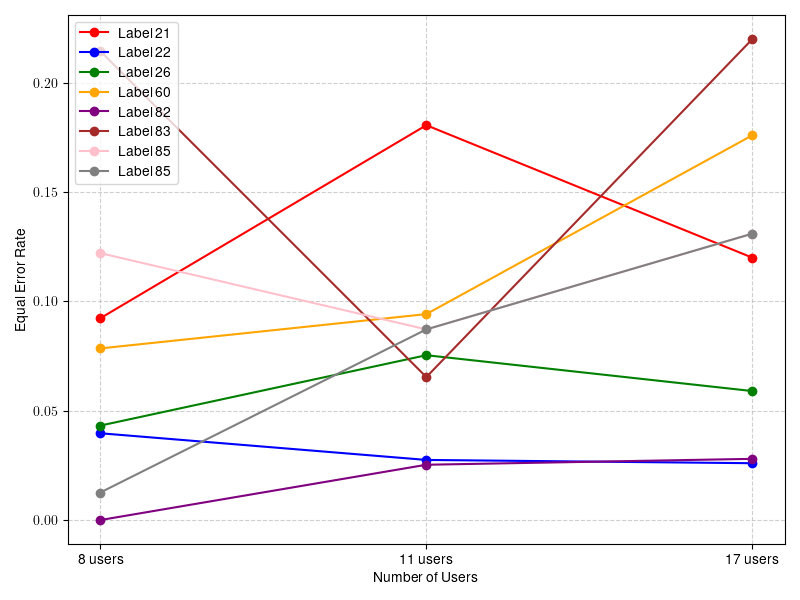
\includegraphics[width=.7\textwidth]{images/subset_test_res.png}
	\caption{"Impact of smaller user subset on EER across 8 models.}
	\label{fig:subset_plot}
\end{figure}

As demonstrated in the figure, the impact of increasing the user subset size varies significantly across models. Notably, for 3 of the 8 tested models, the relationship was non-monotonic. Consequently, drawing definitive conclusions from this test is challenging due to the limited number of data points.

\subsection{Two-Model Test}
This small-scale test can be considered an extreme version of the subset test, reduced to include only two models. The purpose of this test was to evaluate whether the proposed solution could reliably differentiate between these two users under optimal conditions.

The results of this test are presented in the figure below.

\begin{figure}[H]
	\centering
	\begin{subfigure}{.5\textwidth}
		\centering
		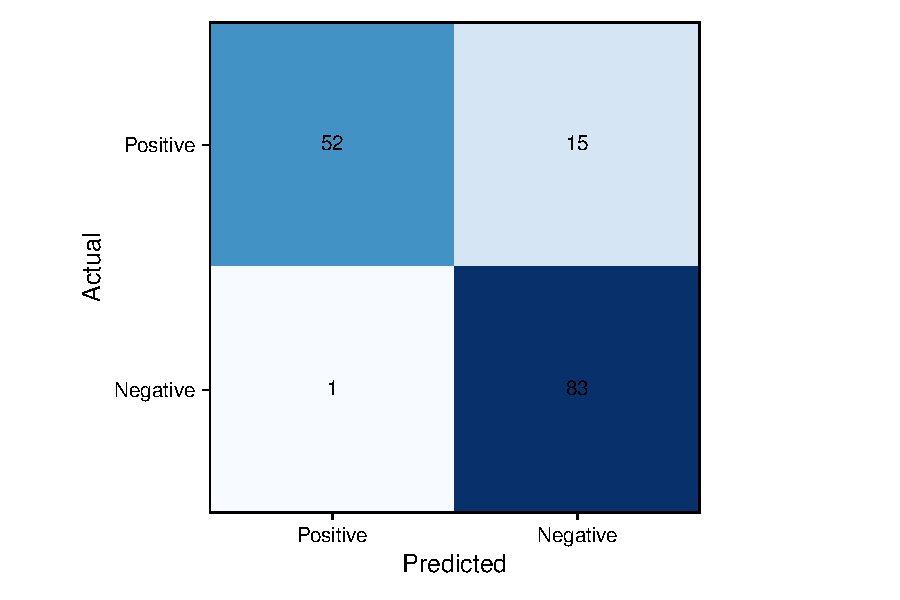
\includegraphics[width=.99\textwidth]{images/confusion_matrix_25.pdf}
		\caption{Confusion matrix for model 25.}
		\label{fig:sub1}
	\end{subfigure}%
	\begin{subfigure}{.5\textwidth}
		\centering
		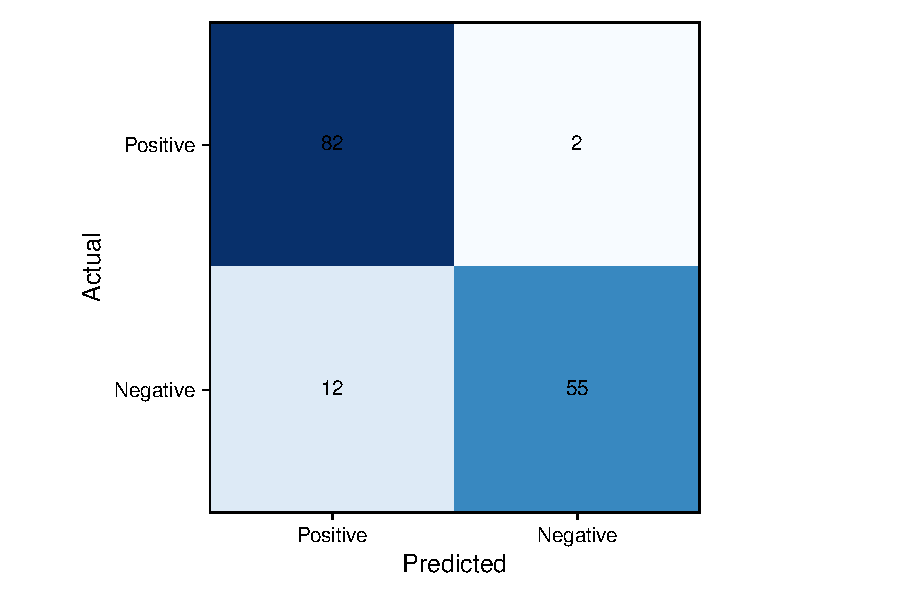
\includegraphics[width=.99\textwidth]{images/confusion_matrix_86.pdf}
		\caption{Confusion matrix for model 86.}
		\label{fig:sub2}
	\end{subfigure}
	\caption{Confusion matrices for models 25 and 86 tested exclusively on their respective datasets.}
	\label{user_vs_user}
\end{figure}

The models trained under these conditions achieved false positive rates of 1.2\% for Model 25 and 21\% for Model 86. These results represent a significant improvement over the baseline models, which demonstrated false positive rates exceeding 60\%, as shown in Figure \ref{fig:all_models_5_len40}.\\
This test demonstrates that the proposed method is capable of distinguishing between these two users when trained under optimal conditions. However, when the models are trained on the full dataset, this ability is substantially diminished.